% !TEX program = xelatex
% DDA5001 HW1 answer paper; the supplied template's layout was adapted without its sample content or images.
\documentclass[11pt,a4paper]{article}
\usepackage{fontspec}
\setmainfont{TeX Gyre Termes}
\usepackage[a4paper,margin=24mm,headheight=16pt]{geometry}
\usepackage{amsmath,amssymb,booktabs,graphicx,xcolor,fancyhdr,lastpage,hyperref,listings}
\definecolor{CoursePurple}{HTML}{5C2267}
\hypersetup{colorlinks=true,linkcolor=CoursePurple,pdftitle={DDA5001 Homework 1}}
\pagestyle{fancy}\fancyhf{}
\fancyhead[L]{\small DDA5001 Machine Learning}
\fancyhead[R]{\small Homework 1}
\fancyfoot[R]{\small\thepage/\pageref*{LastPage}}
\setlength{\parindent}{1.2em}\setlength{\parskip}{3pt}
\newcommand{\R}{\mathbb R}
\newcommand{\Ein}{E_{\rm in}}
\begin{document}
\begin{center}{\Large\bfseries\color{CoursePurple}DDA5001 Homework 1}\\[4pt]
The Chinese University of Hong Kong, Shenzhen\\[2pt]
\small Kunyuan Zhong \quad Student ID: 226040255\end{center}
\noindent\rule{\linewidth}{0.8pt}

\section*{Problem 1: Concepts and fundamental knowledge}
\textbf{(a)} Supervised learning uses examples with target labels or values to learn a mapping from inputs to targets. Unsupervised learning uses inputs without such targets to discover structure, such as clusters or lower-dimensional representations.

\textbf{(b)} Statement 2 is true. When $n<d$, $\operatorname{rank}(X)\leq n<d$, so $\ker(X)$ contains a nonzero vector. If $\hat\theta$ minimizes least squares, so does $\hat\theta+v$ for every $v\in\ker(X)$; there are infinitely many minimizers. Regression ordinarily fits numerical targets, a perceptron need not have a unique separating solution, and least squares is not an MLE for every noise distribution.

\textbf{(c)} For every nonzero $v\in\R^d$, full column rank means $Xv\neq0$. Hence $v^\top X^\top Xv=\|Xv\|_2^2>0$. Therefore $X^\top X$ is positive definite and invertible, giving a unique least-squares minimizer. The Hessian of $\|X\theta-y\|_2^2$ is $2X^\top X\succ0$, so the objective is strongly convex.

\section*{Problem 2: Least squares without full column rank}
\textbf{(a)} Write the supplied SVD as $X=V\Sigma_1U_1^\top$ and complete $U_1$ with $U_2$ to an orthogonal basis of $\R^d$. Because $\Sigma_1$ is invertible, minimizing $\|V\Sigma_1z-y\|_2^2$ over $z=U_1^\top\theta$ gives $z^*=\Sigma_1^{-1}V^\top y$. Thus all solutions are
\[\boxed{\theta=U_1\Sigma_1^{-1}V^\top y+U_2w,\qquad w\in\R^{d-n}.}\]
Indeed $U_1^\top U_2=0$, and $U_2w$ spans $\ker(X)$. Since $\operatorname{rank}(X)=n$, $X$ is onto $\R^n$; every listed solution satisfies $X\theta=y$, and the optimal value is $0$.

\textbf{(b)} Differentiating the regularized objective yields $2X^\top(X\theta-y)+2\lambda\theta=0$. Since $v^\top(X^\top X+\lambda I)v=\|Xv\|_2^2+\lambda\|v\|_2^2>0$ for nonzero $v$, the unique solution is
\[\boxed{\theta_\lambda=(X^\top X+\lambda I)^{-1}X^\top y.}\]
The inverse is a theoretical expression; a numerical implementation should solve the linear system.

\section*{Problem 3: Robust linear regression}
\textbf{(a)} For residuals $r_i=(X\theta-y)_i$, the i.i.d. Laplace likelihood gives
\[-\log p(y\mid X,\theta)=n\log(2b)+\frac1b\sum_{i=1}^n|r_i|.\]
Both $n\log(2b)$ and the positive factor $1/b$ do not affect the minimizer in $\theta$. The MLE therefore minimizes $\sum_i |(X\theta-y)_i|$.

\textbf{(b)} For the specified shifted smoothing,
\[
h'_\mu(z)=\begin{cases}-1&z\leq-\mu,\\z/\mu&|z|<\mu,\\1&z\geq\mu,\end{cases}
\qquad \nabla L(\theta)=X^\top g(X\theta-y),
\]
where $X\in\R^{n\times d}$, $X\theta-y,g(X\theta-y)\in\R^n$, and $\nabla L(\theta)\in\R^d$. The branches agree at $\pm\mu$. Here $h_\mu(0)=\mu/2$; the implemented objective is a sum.

\textbf{(c)} The supplied $n=1000,d=50$ data were used with $\mu=10^{-5}$, $\alpha=0.001$, $T=1000$, and \texttt{default\_rng(0)}. Numerical least squares gave $\|\hat\theta_{\rm LS}-\theta^*\|_2=59.51363648$. The Huber descent error changed from $8.98993999$ at $k=0$ to $5.61872016$ at $k=1000$; its sum loss changed from $256704.09771$ to $252724.64378$. The code loads $\theta^*$ only after fitting to calculate these errors. Figure~\ref{fig:p3} uses all 1001 recorded states; the objective and errors are in \texttt{regression\_history.csv}.
\begin{figure}[htbp]\centering
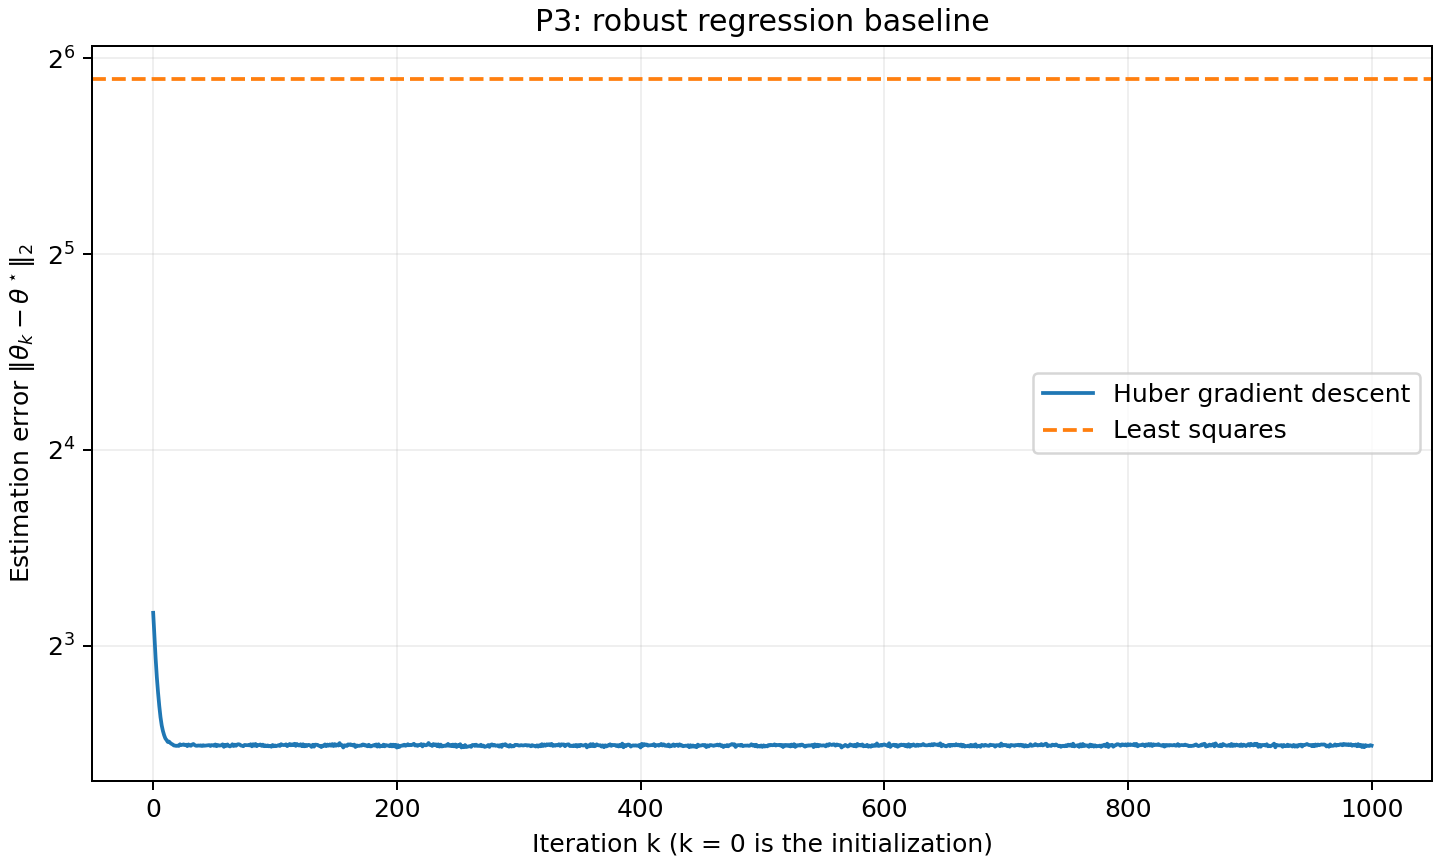
\includegraphics[width=.78\linewidth]{../results/p3-baseline-20260929/regression_error.png}
\caption{P3 parameter error versus update count, with the least-squares reference.}\label{fig:p3}
\end{figure}

\textbf{(d)} The scalar check at $z/\mu=(-2,-0.5,0,0.5,2)$ returned $h'_\mu(z)=(-1,-0.5,0,0.5,1)$ for both tested values of $\mu$. The small matrix gives $\nabla L=(0.5,1.0)^\top$ and $\nabla L^\top v=1.1$. Selected central differences are shown below; the full values are in \texttt{gradient\_verification.csv}.
\begin{center}\small
\begin{tabular}{@{}rrrrr@{}}\toprule
$\mu$&$t/\mu$&sum difference&mean difference&$|D_tL-1.1|$\\\midrule
$1$&$1$&$0.7625$&$0.1525$&$0.3375$\\
$1$&$0.1$&$1.1000$&$0.2200$&$1.33\times10^{-15}$\\
$1$&$10^{-4}$&$1.100000000003$&$0.220000000001$&$2.77\times10^{-12}$\\
$10^{-5}$&$1$&$0.7625$&$0.1525$&$0.3375$\\
$10^{-5}$&$0.1$&$1.1000$&$0.2200$&$6.66\times10^{-16}$\\
$10^{-5}$&$10^{-4}$&$1.100000000002$&$0.220000000000$&$2.41\times10^{-12}$\\\bottomrule
\end{tabular}\end{center}
The first-order Taylor formula $L(\theta+tv)=L(\theta)+t\nabla L(\theta)^\top v+o(t)$ explains convergence of the loss-change ratio to $1.1$. At $t/\mu=1$, the step is too large for a local approximation and crosses branches. Tiny steps can amplify subtraction roundoff; the supplied $10^{-4}\mu$ steps still give small absolute errors, so the table does not claim an observed failure at that size. The mean gradient is $(0.1,0.2)^\top=\nabla L/5$ and its directional derivative is $0.22$. To make $\theta-\alpha_{\rm sum}\nabla L$ equal to a mean-gradient update, use $\alpha_{\rm mean}=5\alpha_{\rm sum}$. The baseline code uses the sum gradient without division by $n$.

\section*{Problem 4: Perceptron convergence}
Assume $\theta_0=0$, and index $k$ by mistake updates.
\textbf{(a)} Each of the finitely many values $y_i\theta^{*\top}x_i$ is strictly positive. Their minimum $\rho$ is therefore positive.

\textbf{(b)} For the example selected at update $k$,
\[\theta_k^\top\theta^*=\theta_{k-1}^\top\theta^*+y_{k-1}x_{k-1}^\top\theta^*\geq\theta_{k-1}^\top\theta^*+\rho.\]
Induction from $\theta_0=0$ yields $\theta_k^\top\theta^*\geq k\rho$.

\textbf{(c)} A mistake under the specified sign convention implies $y_{k-1}\theta_{k-1}^\top x_{k-1}\leq0$ (equality can arise for a negative label). Consequently,
\[\|\theta_k\|_2^2=\|\theta_{k-1}\|_2^2+2y_{k-1}\theta_{k-1}^\top x_{k-1}+\|x_{k-1}\|_2^2\leq\|\theta_{k-1}\|_2^2+\|x_{k-1}\|_2^2.\]

\textbf{(d)} Since each $\|x_i\|_2\leq R$, induction gives $\|\theta_k\|_2^2\leq kR^2$.

\textbf{(e)} For $k\geq1$, combining (b) and (d) gives
\[\frac{\theta_k^\top\theta^*}{\|\theta_k\|_2}\geq\frac{\sqrt{k}\rho}{R}.\]
Cauchy--Schwarz bounds the left side above by $\|\theta^*\|_2$. Hence every possible mistake count obeys $k\leq R^2\|\theta^*\|_2^2/\rho^2$; the algorithm cannot continue making mistakes beyond this finite bound. This concerns mistake updates on strictly separable data, not epochs or a nonseparable sample.

\section*{Problem 5: Perceptron and pocket}
\textbf{(a)} The features are mean intensity and mean absolute left--right asymmetry of each $16\times16$ image, with input $(1,\text{intensity},\text{asymmetry})^\top$. The code predicts $+1$ at score zero. It updates the current weights by $\theta\leftarrow\theta+yx$ at a uniformly sampled current mistake. The pocket stores a separate copy only if the new training error is strictly smaller; ties retain the earlier pocket. Training never reads test labels. The run used seed 0 and 2000 mistake updates.

\textbf{(b)} The filtered data contain 1669 training and 434 test images. At update 2000, current train/test errors are $0.04014380/0.07142857$ and pocket train/test errors are $0.03235470/0.06451613$. Figure~\ref{fig:p5curves} and \texttt{trajectory.csv} show the full trajectory. Pocket training error equals the running minimum of current training error and had zero increases. Current training error fluctuated. The pocket test curve rose twice during this run even though its final value is below the current test error; no test monotonicity follows from selection on training error.
\begin{figure}[htbp]\centering
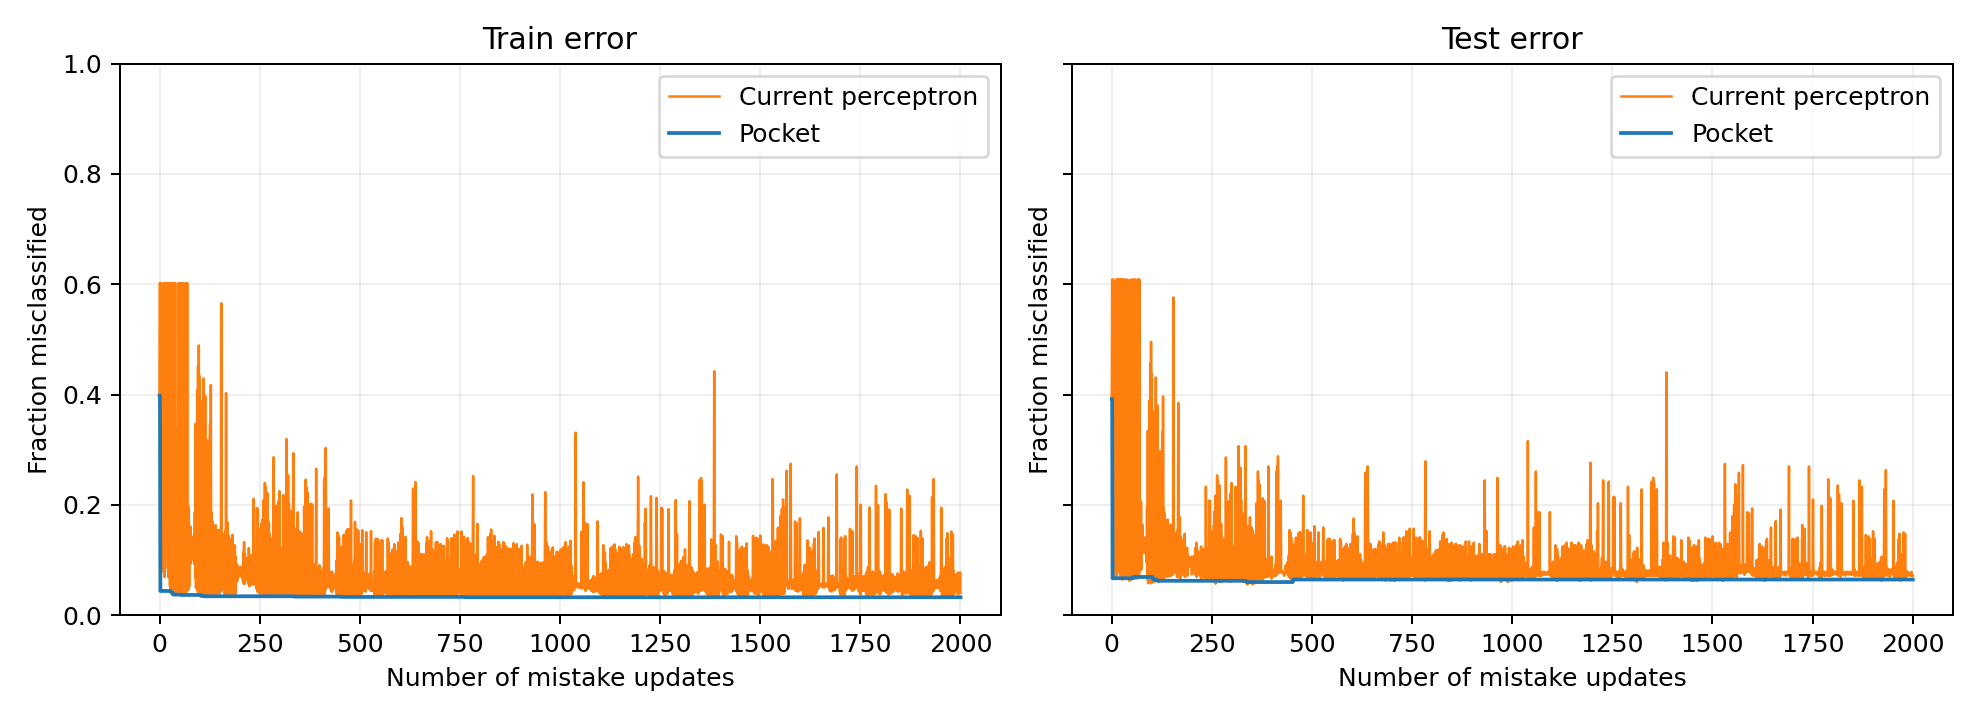
\includegraphics[width=.82\linewidth]{../results/p5-baseline-20260929/error_curves.png}
\caption{P5 current and pocket errors on training and held-out data.}\label{fig:p5curves}
\end{figure}

\textbf{(c)} Figure~\ref{fig:p5boundary} uses 500 training images from each class and overlays the two final boundaries. The bias weight is the intercept of the score $\theta_0+\theta_1\,\text{intensity}+\theta_2\,\text{asymmetry}$, allowing a boundary away from the feature-space origin. The supplied plotting routine handles a vertical boundary when $\theta_2=0$ and a constant classifier when both feature weights are zero.
\begin{figure}[htbp]\centering
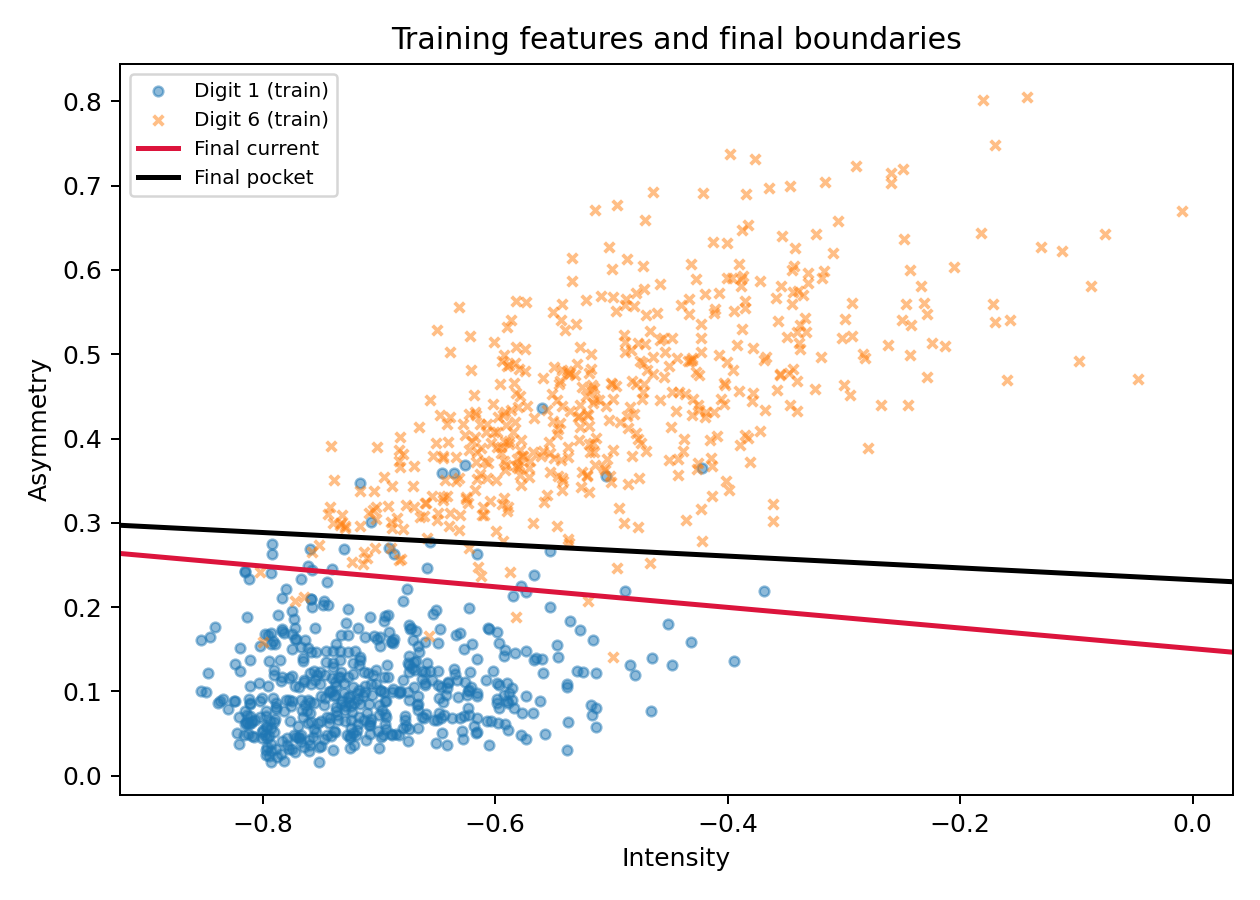
\includegraphics[width=.64\linewidth]{../results/p5-baseline-20260929/decision_boundaries.png}
\caption{P5 training features and final current and pocket decision boundaries.}\label{fig:p5boundary}
\end{figure}

\textbf{(d)} Before running the check, we expected the pocket training error to be nonincreasing and equal the running minimum of current training errors. We did not expect this for test error. In the seven-row toy trace:
\[
\begin{aligned}
\Ein(\theta_k)&=(.50,.50,.25,.50,.25,.50,.25),\\
\Ein(\hat\theta_k)&=(.50,.50,.25,.25,.25,.25,.25).
\end{aligned}
\]
At update 2, current weights $(0,-1,0)$ predict $+1$ for the first three samples and $-1$ for the fourth, so only sample 2 is wrong: $\Ein=1/4$. Because this improves on $1/2$, the pocket copies these weights. At update 3, current weights $(-1,-1,0)$ make two errors, so the pocket remains $(0,-1,0)$. The audit compared every saved pocket error to the cumulative minimum of current errors and recomputed errors from saved weights. Copying matters because an in-place change to an aliased current array would silently change the stored pocket. A temporary pocket test-error rise alone is compatible with this training-only selection rule.

\section*{Reproduction notes}
\begingroup\small
Actual command invocations from repository root \path{/home/scarramcci/Project/MCS_CUHK-SZ} are below; shell redirections to logs are omitted. Runtime: CPU, \path{/usr/bin/python3} 3.14.4, NumPy 2.3.5, Matplotlib 3.10.7. All runs used seed 0. P3 used $\mu=10^{-5}$, $\alpha=0.001$, $T=1000$; P5 used 2000 updates, and the toy audit used six.
\lstset{basicstyle=\ttfamily\scriptsize,breaklines=true,breakatwhitespace=false,columns=fullflexible}
\begin{lstlisting}
MPLCONFIGDIR=/tmp/dda-mpl /usr/bin/python3 DDA5001_Machine_Learning/assignments/hw01/src/p3.py --verify-only --output-dir DDA5001_Machine_Learning/assignments/hw01/results/p3-verify-20260929
MPLCONFIGDIR=/tmp/dda-mpl /usr/bin/python3 DDA5001_Machine_Learning/assignments/hw01/src/p3.py --data-dir DDA5001_Machine_Learning/assignments/hw01/requirements/code_source/code_source/p3/data --output-dir DDA5001_Machine_Learning/assignments/hw01/results/p3-baseline-20260929
MPLCONFIGDIR=/tmp/dda-mpl /usr/bin/python3 DDA5001_Machine_Learning/assignments/hw01/src/p5.py --audit-only --output-dir DDA5001_Machine_Learning/assignments/hw01/results/p5-audit-20260929
MPLCONFIGDIR=/tmp/dda-mpl /usr/bin/python3 DDA5001_Machine_Learning/assignments/hw01/src/p5.py --train-data DDA5001_Machine_Learning/assignments/hw01/results/input-conversion-20260929/train_data.npz --test-data DDA5001_Machine_Learning/assignments/hw01/results/input-conversion-20260929/test_data.npz --output-dir DDA5001_Machine_Learning/assignments/hw01/results/p5-baseline-20260929
\end{lstlisting}
All four exited 0. P5 used \texttt{.npz} copies converted from teacher \texttt{.mat} arrays by SciPy 1.18.1 (Python 3.12.14); independent elementwise comparison found maximum difference 0. Teacher inputs are not in the ZIP. The listed commands ran in the working checkout. To run the extracted scripts, unpack the separately supplied \path{code_source.zip}: point P3's \texttt{--data-dir} to \path{code_source/p3/data}, and P5's \texttt{--train-data}/\texttt{--test-data} to \path{code_source/p5/train_data.mat}/\path{test_data.mat} in a NumPy/SciPy/Matplotlib environment. This is a reuse instruction, not another performed run.
\endgroup
\clearpage
\section*{Problem 3(e): AI collaboration case}
\noindent\textbf{Tool and prior expectation.} I used Codex (GPT-6 Astra, as displayed in the conversation interface) to complete the mathematical TODOs in \texttt{src/p3.py} and interpret checks. Before any verification run, the conversation recorded this expectation: the sum-loss gradient should agree with a small directional finite difference; the mean-loss gradient should be the sum gradient divided by $n$; too large or too small a step may enlarge numerical error. This was a prediction, not a measured result.

\noindent\textbf{Two actual result-based follow-ups.} First, I sent \texttt{huber\_branches.csv} values and asked whether the implementation exactly matched the sum of shifted Huber losses, including $z=0$ and both outer branches. The agent checked $h_\mu(0)=\mu/2$, the outer values and derivatives, and \texttt{np.sum}, then replied that no code change was needed. Second, I returned rows from \texttt{gradient\_verification.csv}: at $\mu=t=10^{-5}$ the central difference was $0.7624999999999995$ versus analytic $1.1$; at $t\approx10^{-6}$ it was $1.0999999999999994$, and the mean-loss difference was $0.2200000000000004$. I asked why the larger step differed and how finite-difference error differs from first-order Taylor loss-change error. The agent explained that a step of size $\mu$ crosses smoothing branches and averages slopes away from the current point. It distinguished $|D_tL-\nabla L^\top v|$ from $|L(\theta+tv)-L(\theta)-t\nabla L^\top v|$. At $t=\mu$ these were $0.3375$ and $1.24\times10^{-5}$; at $t=0.1\mu$ they were approximately $6.66\times10^{-16}$ and $1.32\times10^{-7}$.

\noindent\textbf{Decision.} I retained the implementation. The code applies the handout's inner formula $z^2/(2\mu)+\mu/2$, outer formula $|z|$, and \texttt{np.sum}; its gradient returns $X^\top g$ without division by $n$. The small-example sum gradient is $(0.5,1)^\top$, while the mean gradient is $(0.1,0.2)^\top$. Their directional derivatives $1.1$ and $0.22$ and the small-step differences agree. The sum-to-mean difference ratio is $5$, as expected for five samples, but that ratio alone follows from dividing one loss by five; branch values and code provide additional evidence. A mean-gradient implementation would need $\alpha_{\rm mean}=5\alpha_{\rm sum}$ for the same small-example update. The original prompts and replies remain in this Codex conversation; full evidence is in the cited CSVs.

\clearpage
\section*{Problem 5(e): AI collaboration case}
\noindent\textbf{Tool and prior expectation.} I used Codex (GPT-6 Astra, as displayed in the conversation interface) for the perceptron and pocket TODOs and their audit. Before verification, the conversation recorded that pocket training error should be the running minimum of current training error and hence nonincreasing; no such guarantee was predicted for test error.

\noindent\textbf{Two actual result-based follow-ups.} I returned the seven-row \texttt{toy\_trace.csv} and asked the agent to recompute the update-2 error and check the strict pocket rule. Its reply checked the four predictions at weights $(0,-1,0)$: the three inputs $(1,0,0)$ have score zero and predict $+1$; the fourth $(1,1,0)$ has score $-1$ and predicts $-1$. Only the second label is wrong, so the error is $1/4$. At update 1 the current error tied the stored $0.5$, so pocket stayed at zero; update 2 improved $0.5$ to $0.25$, so it copied the new weights; update 3 raised current error to $0.5$, so pocket remained at $0.25$. I later returned two rises from \texttt{trajectory.csv}: at update 54, pocket train/test errors changed $0.037148\to0.036549$/$0.066820\to0.069124$; at update 453, they changed $0.033553\to0.032954$/$0.059908\to0.064516$. The agent checked that each new current training error was strictly below the previous pocket error and that pocket copied the new weights.

\noindent\textbf{Decision.} I retained the code. Its comparison uses only training error, so rises in held-out error do not violate the pocket guarantee. In the toy trace the pocket sequence $(.5,.5,.25,.25,.25,.25,.25)$ equals the running minimum of current errors. The full trajectory audit checks this equality for every saved state. Test labels are loaded and used to score saved weights only after training finishes. Copying the pocket array prevents a later in-place current update from changing the stored best state. The original prompts and replies remain in this Codex conversation; the CSVs contain the numeric evidence.
\end{document}
